\documentclass[12pt]{article}
\usepackage{mystyle}
\usepackage[T1]{fontenc}
%\usepackage{mathptmx} % times new roman 
\usepackage{tgpagella} % tgpagella

\title{ECON899. 
Problem set 1}
\author{Emily Case, Hanna Han, Anna Lukianova}
\date{}

\begin{document}

\maketitle

\section{Problem}
Agents solve 
\begin{align*}
    V(K,Z) & = \max_{K', C} \log(C) + \beta \mathbb{E}[V(K', Z')|Z] \\
    & \quad \text{s.t. } C = ZK^\theta + (1-\delta)K - K' \\
    & = \max_{K'}\; \log(ZK^\theta + (1-\delta)K - K') + \beta \left[ Pr(Z' = Z^g |Z) V(K', Z^g) + Pr(Z'= Z^b | Z) V(K', Z^b)\right]
\end{align*}
Where $Z^g = 1.25$ and $Z^b = 0.2$ with the following transition matrix:
\begin{align*}
    \Pi & = \begin{bmatrix}
        0.977 & 0.023 \\
        0.074 & 0.926 \\
    \end{bmatrix}
\end{align*}

\section{Results}
\subsection*{Q2.}
Our results and graphs are coming from our Julia code. For each value of $Z$ the value function is indeed increasing in capital $K$ (Figure \ref{F1}, left). It is also concave in capital since the value function changes are decreasing in capital.
\begin{figure}
    \centering
    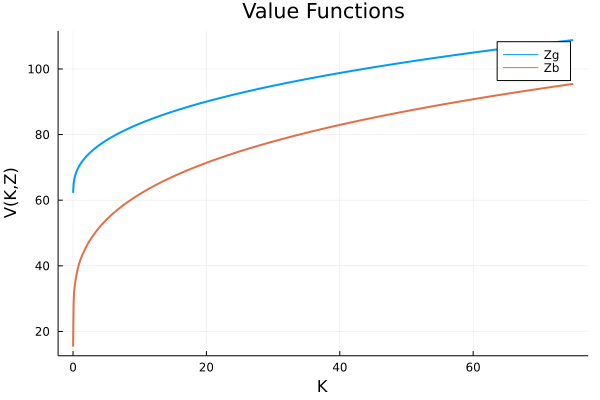
\includegraphics[width = 0.45\linewidth]{pset1/figures/valfunctions.png}
    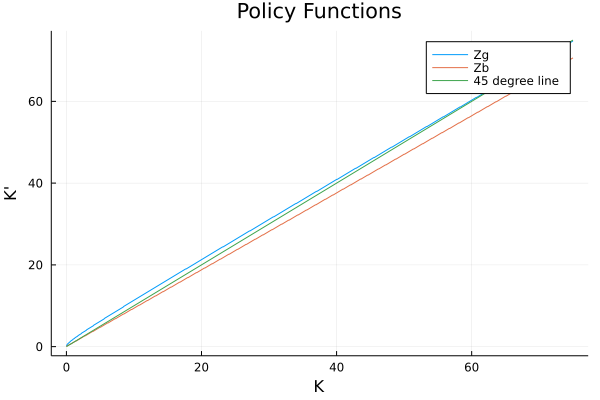
\includegraphics[width = 0.45\linewidth]{pset1/figures/polfunctions.png}
    \caption{Value and policy functions for good and bad technology shocks.}
      \label{F1}
\end{figure}

\subsection*{Q3.}

\begin{figure}
    \centering
    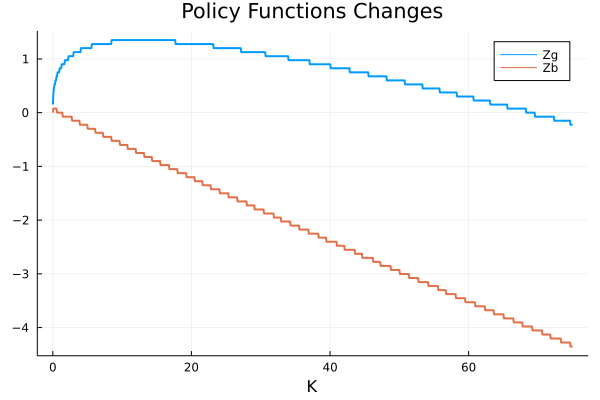
\includegraphics[width = 0.5\linewidth]{pset1/figures/polfuncchanges.png}
        \caption{Changes in the policy functions for good and bad technology shocks.}
      \label{F2}
\end{figure}

 The decision rules are also increasing in $K$ and $Z$ (Figure \ref{F1}, right). 

We also calculate the change in the decision rules $K'(K,Z) - K$ for both states of $Z$ (Figure \ref{F2}). We find that the savings is a decreasing function in the current capital level for the bad shock realization, while for the good shock realization it is a non-monotonic function in capital. The savings is an increasing function in the productivity shock, and in good conditions people want to invest more in tomorrow's capital, especially at low values of capital. % idk if this is correct.

\subsection*{Comparing times}
% to go somewhere: (these numbers might not be up to date) 
Julia solves the model in 2.042580755 seconds, and with parallelizing julia solves the model in 3.450236762 seconds. Fortran solves the model in 362.828003 seconds. It seems to take too much time. Probably, our Fortran code is inefficiently written. The results obtained from Fortran coincides with the results from Julia.
%%% Do we need to add plots?

\end{document}